\subsection {Holographic Emulation}
\label{sec.holographic_emulation}

The proposal of this work is to investigate a VR environment that can provide the combined effects of the hologram but that don't have the computational cost of CGH. Most of current VR environments can be composed of off-the-shelf hardware, and the proposed environment does not rely on specialized hardware for CGH to avoid the its high costs~\cite{fournier2004}. The proposed VR environment is composed by two 3D standard stereo TVs, combined in a Fish Tank Virtual Reality (FTVR)~\cite{Ware1993} environment and a depth camera. The camera creates a Head Coupled Perspective (HCP)~\cite{okoshi2012}, as shown in Figure~\ref{fig.tv_setup}a, by projecting virtual objects considering the location of the viewer, which is acquired by tracking. HCP improves the depth perception~\cite{li2012} and, when combined with stereo vision, can create an holographic emulation. 

The FTVR is combined with HCP and stereo vision to create a virtual screen, which is the perceived screen from the depth cues created by the two stereo displays that are juxtapositioned with a tilt angle of $120^{\circ}$ in Figure~\ref{fig.tv_setup}a. The surround viewing is achieved by tracking the position of the viewer as in the original FTVR setup. Although HCP is has been reported more important than stereo in 3D visualization~\cite{Ware1993}, the holographic perception is created using the binocular parallax. The HCP viewing is adjusted with negative parallax to create the depth cue of the virtual screen and the spectral illusion of Pepper's Ghost. Other depth cues are adjusted to the viewing angle of the virtual screen using the position tracked by the the depth camera.

\begin{figure}[!hbt]
\centering
\begin{tabular}{cc}
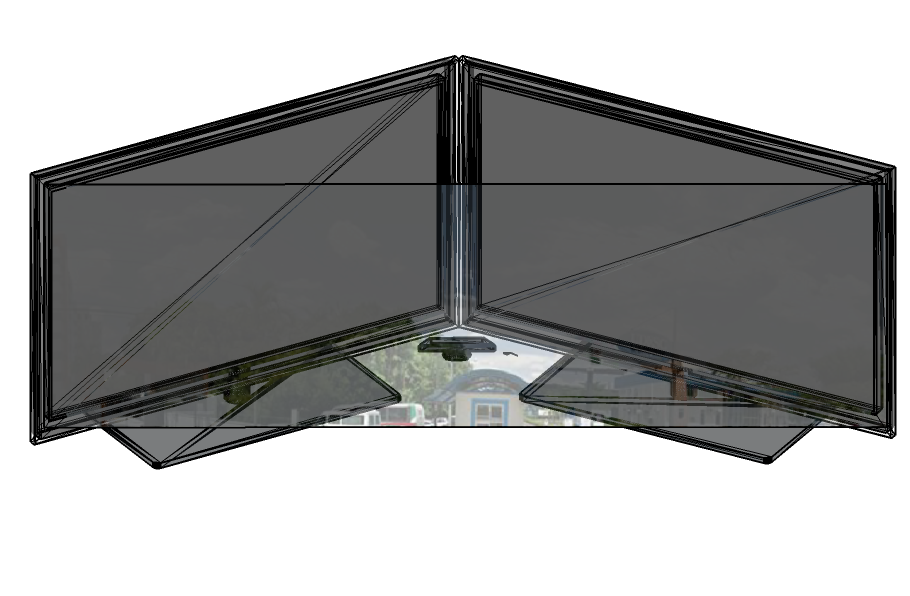
\includegraphics[width=0.4\linewidth,keepaspectratio=true]{figs/labsetup_01.png}&
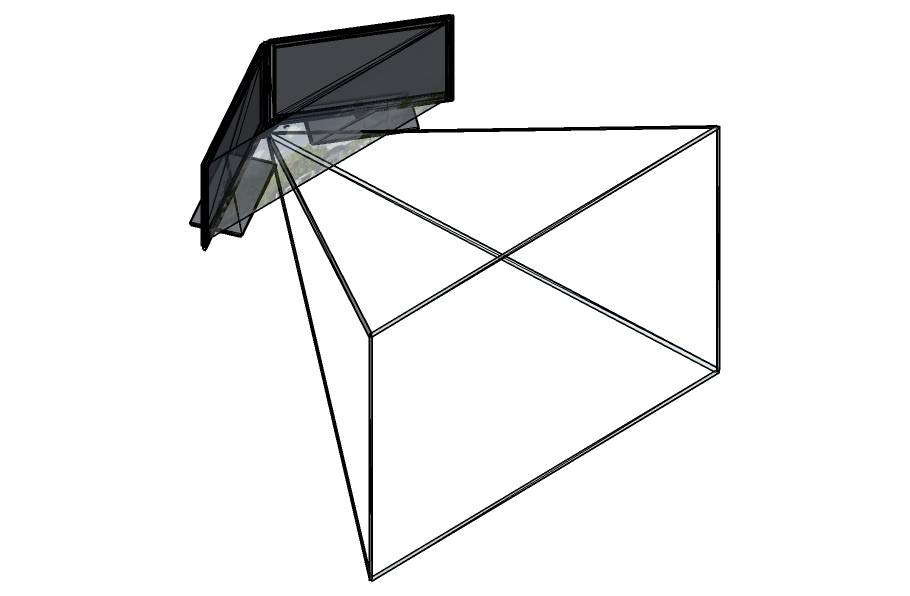
\includegraphics[width=0.4\linewidth,keepaspectratio=true]{figs/labsetup_02.png}\\
(a) Virtual screen & 
(b) Tracking frustum
\end{tabular}
\caption{FTVR setup of the stereo displays and Kinect.}
\label{fig.tv_setup}
\end{figure}

The tracking system has to capture the position of the viewer with high accuracy in order to avoid incorrect HCP. It also needs to be robust to body movement or objects that may partially occlude the viewer. In order to achieve the desired robustness and accuracy, a depth camera is used instead of a standard RGB camera. The depth sensor has a higher accuracy in the estimation of the depth and with this information can remove artifacts in the image that are occluding or degrading the positional information of obtained from the RGB channels. 

Although the proposed emulation has the restriction of a single viewer for simplicity, the proposed setup can be extended up to four viewers. The depth information can be also used to distinguish two people in front of the TVs, and two depth cameras can be combined to track four viewers. The standard stereo TVs with $240Hz$ refresh rate can provide stereo pairs up to four viewers with some flickering~\cite{Frohlich2005}. 

%This investigation setups two 3D displays forming the FTVR as in the illustration of Figure~\ref{fig.tv_setup}a. 



%The cornerstone of the proposed projection is how this can be done with the existing viewing pipeline of 3D graphics frameworks such as OpenGL. The existing viewing transformations works well for 3D with positive stereo parallax, showing the object as inside the screen of display. In the opposite case, the projection with negative parallax requires the translation $T_{parallax}$ of the scene towards the virtual display. This is incorporated in the view transformation $M_{view}$ of Section~\ref{sec.projection_review}, creating a translated view $M_{view}T$. Let the modification of the viewpoint produce a new view transform $M^{\prime}_{view}$. This new viewpoint combined with $T_{parallax}$ is then defined as $M^{\prime}_{view} T$. The following projection $M_{projection}$ depends on the value of $z$, which means that the latter translation is not applied not only in the depth, but also in the other directions, moving the scene coordinates with the distance from the screen. 

%In the proposed hologram emulation, the scene should be projected with negative parallax to appear in a distance away from the screen. For the viewer, objects of the scene appears in a fixed position outward from the screen. The immersion depends on the viewer position for eye accommodation, stereo convergence and binocular parallax. Additionally to that, the FOV provided by the FTVR and HCP projection enhances the realism of the scene and the sense of presence~\cite{Hounsell2013}. 

%The HCP projection of the scene provided by the OpenGL pipeline in Section~\ref{sec.projection_review} works for standard stereo projection. In the proposed hologram emulation, the projection has to emulate a virtual Volume Of Interest (VOI) with the stereo negative parallax. The VOI is created with depth cues to emulate the hologram. The perspective cue is dependent on the viewing angle and distance from screen, but not on binocular parallax. 

%There is no motion parallax in the VOI and all objects in the hologram have fixed position.

%The main pipeline of OpenGL follows the sequence of transforms: $M_{model}$, $M_{view}$, $M_{proj}$ and $M_{screen}$. In ordinary HCP, $M_{model}$ setups the scene. $M_{view}$ applies the viewpoint from the tracked position, and $M_{proj}$ sets the depth cues. While the perspective depth cue is set with $M_{proj}$, the binocular parallax is set with the stereo projection of Equation~\ref{eq.stereo_projection_matrix} in Section~\ref{sec.stereo_projection}. This projection has zero parallax for a convergence point in the plane of projection, which is the screen of display, and negative parallax at any convergence point in front of the stereoscopic displays. In order to achieve this, the view transform $M_{view}$ has to create a viewpoint looking towards $-z$, because the horizontal negative parallax has to increase away from the screen with the multiplication of the first term on the right of Equation~\ref{eq.stereo_projection_matrix} and the object coordinates $(x, y, z)$ in the VOI. The result of this multiplication is the coordinate translated in $x$ to create the stereo offset, $(x+ sh_z \cdot z, y, z)$. Therefore, the objects have increasing negative parallax in the increasing positive $z$ axis.

%This projective setup introduces a motion parallax for object that are off-center. This is desired for HCP with positive parallax, but not for the hologram emulation because the VOI does not have motion parallax associated with the viewpoint. If $M_view$ is restricted to invert the orientation of the $z$ axis, and $M_{proj}$ applies the shift in the frustum that aligns that origin with the plane with zero parallax, the far plane in most cases, the motion parallax of the HCP is removed. This also is incorrect  because $M_{view}$ should be applied after the shift to generate the viewpoint for HCP. If applied before, the viewpoint is for a scene that is projected along $-z$ as in glFrustum(). One possible way is to correct to keep $M_{view}$ fixed and adjust the rotation and position of each model $M_{model}$ in order to produce the correct viewing angle, but those are cumbersome operations that are not in the semantics of each transform in the OpenGL pipeline. 

%The Figures~\ref{fig.transformation}a-d show an example of a scene composed of duck 3D model. Figure~\ref{fig.transformation}a shows the scene with the shift its applied before the projection to create negative parallax. If the viewpoint is changed to look the top left corner of the picture, a motion parallax is created, illustrated in Figure~\ref{fig.transformation}b. If the shift is applied after $M_{proj}$, the motion and binocular parallaxes are correct, but not the HCP, and the duck in Figure~\ref{fig.transformation}c is not aligned with the viewpoint in the left top corner.The correct viewing angle, as shown in Figure~\ref{fig.transformation}d, can be adjusted programmatically with $M_{model}$ of each object in the scene.

% remove \iffalse ... \fi block to uncomment
\iffalse

\begin{figure}
\centering
\begin{tabular}{|c|c|}
\hline
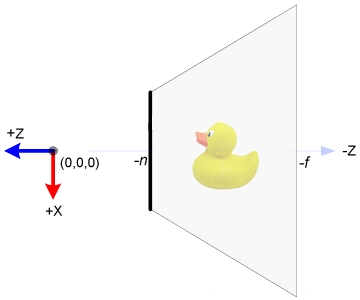
\includegraphics[width=0.45\linewidth,keepaspectratio=true]{figs/scene01.png}
&
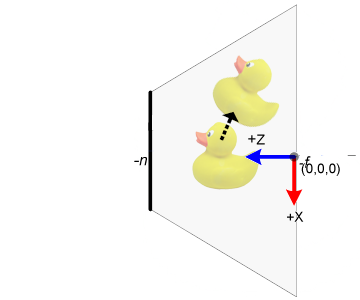
\includegraphics[width=0.45\linewidth,keepaspectratio=true]{figs/scene02.png}
\\
(a)&(b)\\ \hline
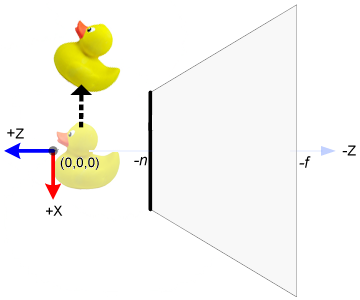
\includegraphics[width=0.45\linewidth,keepaspectratio=true]{figs/scene03.png}
&
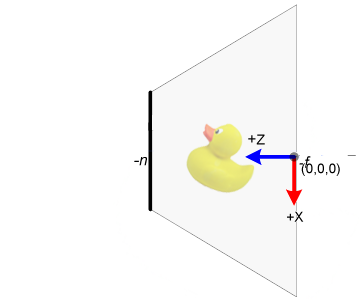
\includegraphics[width=0.45\linewidth,keepaspectratio=true]{figs/scene04.png}
\\ 
(c)&(d)\\ \hline
\end{tabular}
\caption{Example of a scene composed by a duck and the projection frustum of Section~\ref{sec.stereo_projection}. The viewer is at left center in picture (a)  and in the top left corner in pictures (b) to (d).}
\label{fig.transformation}
\end{figure}
\fi






